\documentclass{article}
\title{Proposta de Projeto\\ {\Large EEL7801}}
\author{Aluno: Carlos Freitas}
\date{24 de Agosto de 2023}
\setlength{\parindent}{4em}
\renewcommand{\figurename}{Figura}
\usepackage[letterpaper,top=3cm,bottom=3cm,left=3cm,right=3cm,heightrounded]{geometry}

\usepackage{graphicx}
\usepackage{indentfirst}
\graphicspath{{images/}}

\begin{document}

\maketitle

\section*{Estrutura do Projeto}

O projeto \textit{monitoring system} feito para a disciplina de
Projeto em Eletrônica I, de código EEL7801, tem como objetivo monitorar
um ambiente específico, através de sensores, eletrônica embarcada e um servidor, de modo
que seja possível registrar, organizar e processar os dados coletados para
cumprir determinados requisitos da finalidade do ambiente.

O projeto será realizado individualmente e tem uma estrutura composta
por dois grandes blocos, constituidos de pequenos submódulos com funções específicas.
Um diagrama que contém uma visão de alto nível do projeto está na figura \ref{fig:diagramtoplevel}.

\begin{figure}[ht]
	\centering
	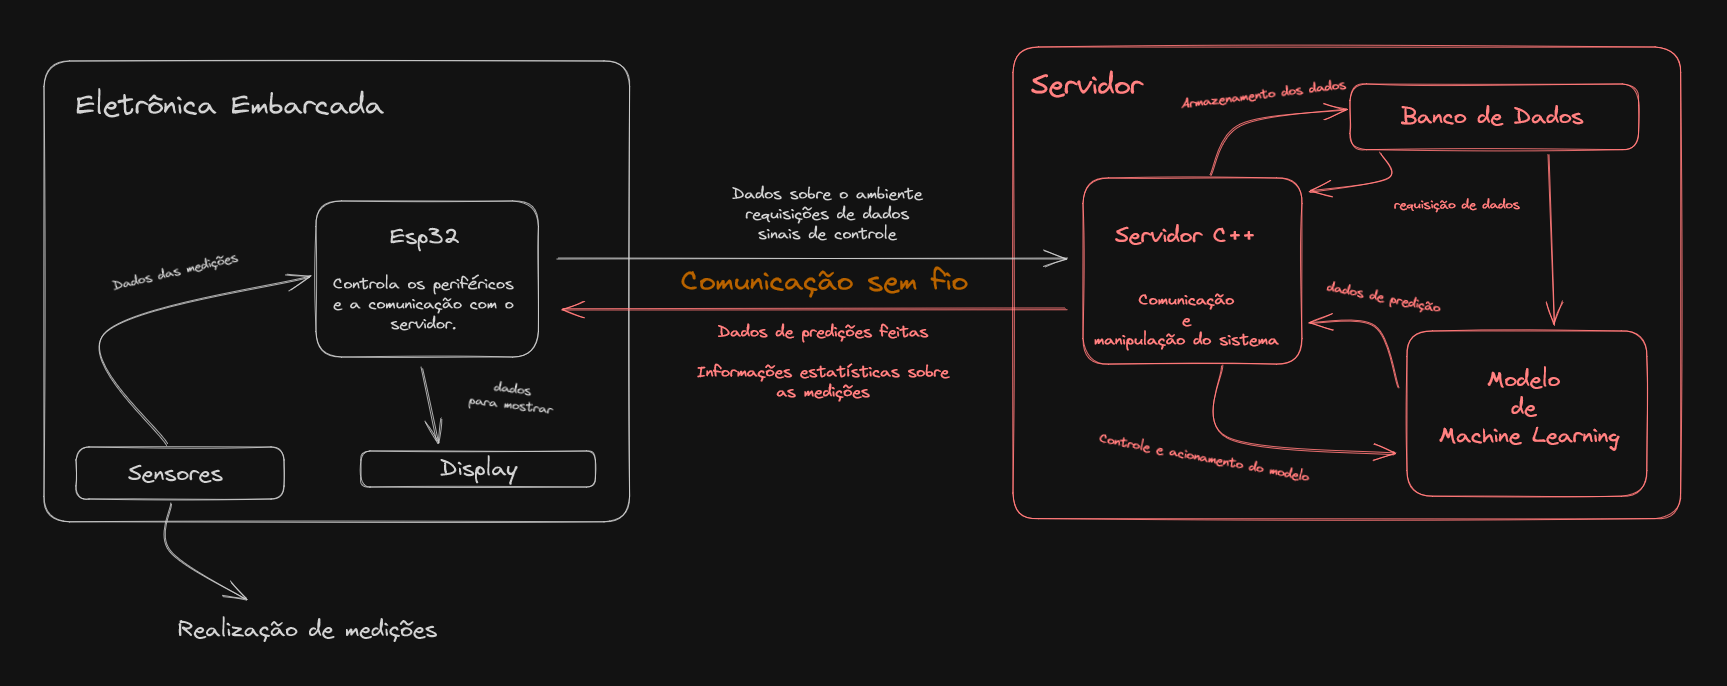
\includegraphics[width=0.85\textwidth,height=6cm]{diagramaprojetoI.png}
	\caption{Diagrama do projeto}
	\label{fig:diagramtoplevel}
\end{figure}

\subsection*{Eletrônica embarcada}

O bloco de eletrônica embarcada, visto na figura \ref{fig:embedded}, é responsável pela leitura das grandezas de interesse,
a exemplo de temperatura, umidade, luminosidade, etc. Tal processo é controlado pelo
microcontrolador central,um esp32, que coordenada a medição realizada pelos sensores. Tendo realizadas as medidas
o esp fará um tratamento nesses dados, de modo a ser mais conveniente de se enviar para o servidor,
além disso, atualizará o display periodicamente com dados atualizados. Há também a comunicação sem fio
com o servidor que será feita pelo microcontrolador, a qual servirá como ponte entre esses dois
blocos, tendo como responsabilidade entregar as requisições do esp32 para o server e controlar a
transferência de dados entre os dois processos.

\begin{figure}[ht]
	\centering
	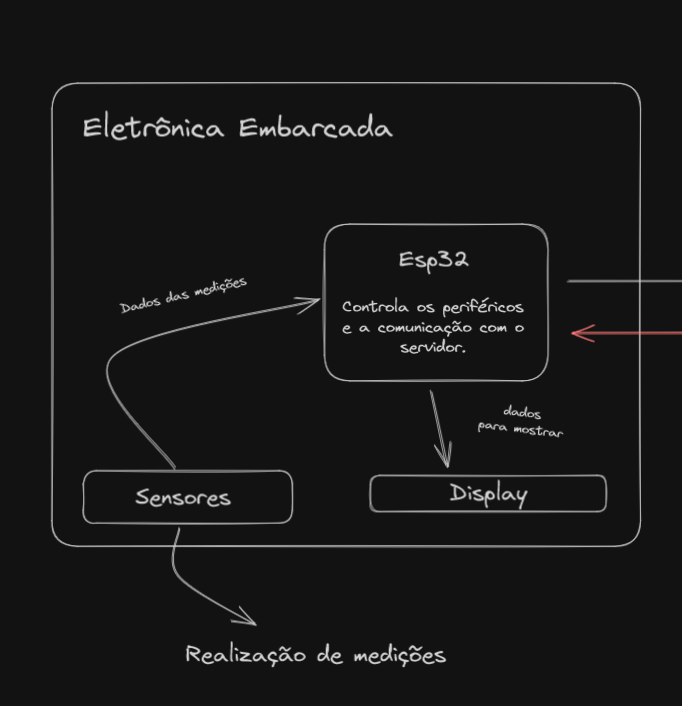
\includegraphics[width=0.85\textwidth,height=5cm,keepaspectratio]{ee.png}
	\caption{Diagrama do bloco de eletrônica embarcada}
	\label{fig:embedded}
\end{figure}

\subsection*{Servidor}

Voltando-se para o segundo grande bloco, ilustrado na figura \ref{fig:server},
tem-se uma subdivisão em três submódulos, um processo principal que controla a comunicação
com o outro bloco e gerencia todas tarefas do servidor, há também um banco de dados para se
armazenar os dados e, finalmente, tem-se uma tarefa específica de
\textit{machine learning} para se criar um modelo que prediz características arbitrárias relevantes.
Um possível exemplo de predição seria a possibilidade chover ou não, baseado nas primeiras leituras de temperatura e
humidade do dia.

\begin{figure}[ht]
	\centering
	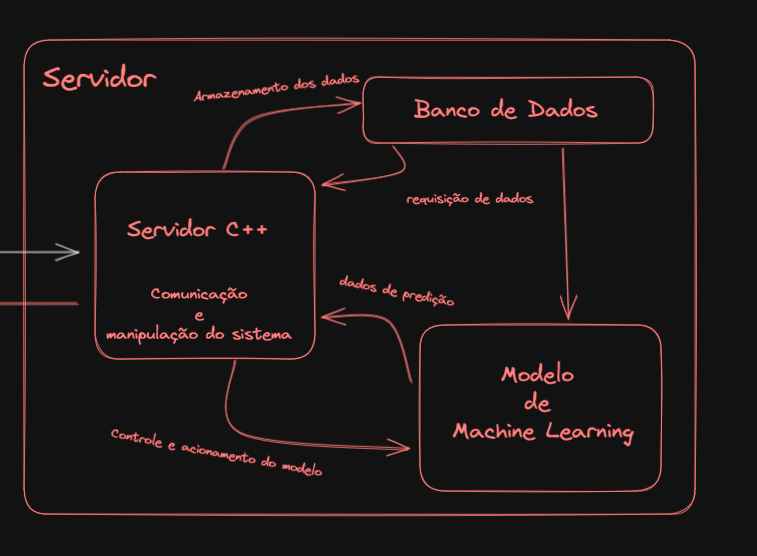
\includegraphics[width=0.85\textwidth,height=5cm,keepaspectratio]{sv.png}
	\caption{Diagrama do bloco do servidor}
	\label{fig:server}
\end{figure}

\end{document}

